\documentclass[9pt,a4paper]{acmproc}
\usepackage[utf8]{inputenc}
\usepackage{amsmath}
\usepackage{amsfonts}
\usepackage{amssymb}
\usepackage{graphicx}
\usepackage[english]{babel}
\usepackage[utf8]{inputenc}
\usepackage{amsmath}
\usepackage{cite}

\graphicspath{}

\author{
  \texttt{Theodor Fleming}
  \and
  \texttt{Andreas Nordberg}
}

\begin{document}
\pagenumbering{gobble}

\title{%
	TDDD66 Projekt \\
	\large WiFi Multicasting}
\maketitle

\clearpage
.
\clearpage

\begin{abstract}
This project explains what multicast, used by WiFi, is, when, how and where it is used and how you as a consumer can take advantage of this knowledge to increase the speed of your home WiFi. The report compares how similar services work and differentiate from each other. It will also briefly cover how the security works when using multicast, and the measures used to block out unwanted receivers of the shared data.
Our conclusion after doing research and performed different tests is that there are some minor things you can do at home to enhance the performance of your WiFi. One way of doing this would be to disconnect the lowest common denominator, the device which slows the network down. 

(To be revised)
\end{abstract}

\clearpage

\section{Inledning}

\subsection{Context}

Multicasting is a method of sharing information by communicating with a select amount of receivers. Other methods exist for this purpose, such as unicast and broadcast, but these will play a lesser role in this study and are only to be compared with multicasting. There are lots of different kinds of networks that uses multicasting to distribute information, but this paper will only focus on how multicasting is handled with WiFi. As with any means of solving a problem, different results can be expected from solving the problem using different methods. In our case with this report, how does WiFi multicasting compare to other means of sharing information within a network in terms of different methods of routing? How well does multicasting do compared to other methods of routing in terms of performance? These are the kind questions this report will delve into and try to answer.  

\subsection{Motivation}

This report will cover why multicasting is a slower service than other communication services of the sort, for example unicast. The following questions then are, what can be done to reduce the discrepancy in speed between the routing methods? How can the throughput in a network be improved with multicast in relation to the other methods of routing. This seems to be an important topic since WiFi data traffic is commonly distributed using multicasting. Our hypothesis is that by increasing the efficiency of how multicasting is handled, the overall speed of the WiFi network would increase.

\subsection{Narrow Scope}

In this study we will do tests and experiments with multicasting using a number of different devices and recievers too see how the speed is altered. Apparently, by using multicasting, the slowest data rate that the slowest reciever can operate with is used and we want to perform experiments on how we can control and change the net speed in the network. Perhaps it is better to disconnect your deprecated phone from your home WiFi network when you aren't using it to not slow down the network using multicast? Our main goal is to see if you as a private user can get faster WiFi by manipulating the speed, options and use of multicast. We hope that the result of this study will help WiFi users how to maximize the speed of your home WiFi network.

\subsection{Methodology}

We will compare the WiFi speed when using different devices, options and recievers. We will also compare the WiFi speed when using multicast and unicast too see if there is a big difference. To achieve this, we will be using some kind of WiFi speed measure application to be able to see what speed the WiFi is operating on and if we can increase the it somehow. 

\subsection{Gameplan}

We are going to do research to understand more how multicast is used, how it works and how we can manipulate it until milestone 2. We need to understand and get a better feel for multicast before we can start with our tests. After that we are going to look into what we can experiment with until milestone 3 and fill the report with more fact about multicast used with Wi-Fi, pros, cons and comparison with other communication services. Now we are going to prepare for the seminar presentation, get feedback and fix the report until final report.

\newpage

\section{Background}

\subsection{What is multicasting?}

While a brief explanation was given in the introduction, we feel like a clarification is needed. With multicasting you are typically referring to the use of multicasting in the network layer protocol, also called IP multicasting. When we started this project, we ourself initially thought that multicasting was the process of multicasting a message on the physical layer, e.g. in our case with WiFi multicasting, perhaps a password-protected network where only the select few connected to the wireless network would be able to decipher and read the outgoing frames sent from the access point out of everyone within the vicinity who could detect them, which would make out a multicast network. This is naturally not how multicasting really works.
\subsubsection*{2.1.1 Unicast}

When you explore Internet you are most likely to use Unicast messaging, it is used when there is a single destination node. 

\begin{figure}[h!]
  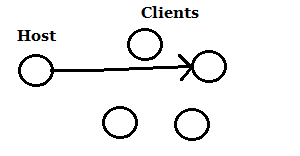
\includegraphics[width=\linewidth]{unicast.png}
  \caption{Unicast}
  \label{fig:Unicast}
\end{figure}

\subsubsection*{2.1.2 Broadcast}

The contrast of Unicast is Broadcast where the destination is all the nodes in the network, often used when your mobile device is searching for a Wi-Fi hotspot.
\begin{figure}[h!]
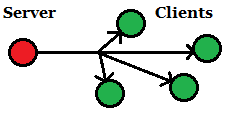
\includegraphics[width=\linewidth]{broadcast.png}
\caption{Broadcast}
\label{fig:Broadcast}
\end{figure}

\subsubsection*{2.1.3 Multicast}





	Multicasting is actually the act of transmitting information in the form of “multicast packets”. These packets are pretty similar to the standard unicast packets, commonly referred to as network packets, but they differ in some ways. While a unicast packet always has one address assigned to a respective receiver, multicast packets have one or more addresses, or a group address which delivers the information to every destination. This is also why multicasting is commonly referred to as “IP multicasting”, because this process is handled at the Network Layer. The perhaps obvious pro to this method of distributing information is that only one sent message or frame is required to share a piece of data to multiple receivers, as opposite to one frame times the number of receivers by using unicasting. A huge chunk of bandwidth can be saved this way, the user can expect its information to be delivered to their device faster and lots of energy and resources can be potentially saved using this method of distribution.
	
	\begin{figure}[h!]
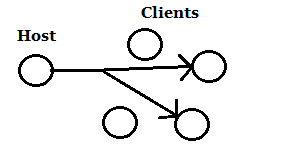
\includegraphics[width=\linewidth]{multicast.png}
\caption{Multicast}
\label{fig:Multicast}
\end{figure}

	These pros sounds great, right? Then why aren’t we using multicasting over the place? Well, multicasting has its cons as well. In our case with WiFi multicasting, while the sender establishes a stable connection with the wireless access point in which the AP acknowledges every received message, the same is not done between the access point and the multiple receivers in the actual multicasting proccess. Much like the UDP protocol, there is no guarantee that a multicasted message is delivered to the designated destination, because the receiver doesn’t reply with any acknowledgement of receiving the given message. Because of this fact, multicasting is most suited for streaming media to a select amount of receivers at a local network. 
	
	There’s also another con to be considered when you’d want to use multicasting in a network. If there is one or more receivers in the multicast network who are slower than the rest of the receivers in the network, for example if this receiver is utilizing a WiFi power saving mode, the entire multicasting network is slowed down to adjust to this one, or more, users. For example, in the case of the power saving mode, several frames are buffered at the access point. DTIM (Delivery Traffic Indicator Message) are then included with the frames to be multicasted, which are a sort of timer of when the access point should release its buffer to all the recipients and not only the ones who have the power save mode enabled. The DTIM included in the frames makes the receivers aware of when to “wake up” from their power saving mode and be ready to receive the buffered batch of frames. \cite{impMult} 
	These pros and cons raises the question of when exactly multicasting would be preferred over unicasting.



\subsection{Multicasting History}

The year was early 1980 and the Stanford University student Steve Deering was tasked with developing a distributed operating system. It was to be called Vsystem and consisted of a few number of computers able to communicate with eachother using a single Ethernet segment. This way the computers could collectively solve tasks together. The system allowed one of the computers in the network to send messages to the rest of the group via MAC layer multicasting. This method of distributing information to several computers at once was nothing short of a success and the need for more computers to be added to this multiprocessing system arose. The problem they faced then was that the other computers available to them was located at the other side of the campus, separated by multiple routers in between the networks. As a result the system had to be extended to allow operation on the layer 3 of the OSI reference model so that the other computers could participate in the multiprocessing system. Steve Deerling then used existing technologies to develop a new distance vector-based multicast routing protocol suited to the system he had imagined, which led into further research about IP multicasting. \cite[s.~7]{briefHist}


\subsection{Experiment}

We are going to use a network simulating program such as Cisco to simulate a network where we compare multicast performance with unicast. The main purpose is to find out approximately how many routers and devices a local network should contain before it is worth implementing multicast instead of unicast. We are going to start in a small scale and see if there is any different in bandwidth depending on either you use multicast or unicast. Then we are successively going to increase the size of the network to see when you reach the point where the multicast technology is using less bandwidth and increasing the speed of the data that is sent within the network.
We also want to try and see if we can create our own multicast network within our home. This could maybe be in favour for example if you have two computers in different parts of your house and you want to play the same song on both simultaneous. We are not really sure on how this is going to be done at this point of time but the basics are that we need to connect these devices over the same IP address. You could compare it with a walkie talkie where everyone on a specific channel can communicate with everyone except in this case the channel is replaced with an IP address. We have to allocate the same a class D IP address to each device in the network that we can call the group address.

\subsubsection{Multicast group}

The device that wants to send and receive multicast datagrams must be in a multicast group. These groups are on a particular network interface and have the IP multicast-address of class D. The range of the D-classified IP address is from 240.0.0.0 to 239.255.255.255. Basically you allocate the device that you want to send and receive multicast datagrams from and to a specific class D address. Now then device knows that if a datagram is sent to that specific IP address it wants to explore it further by sending it up to the next layer. And same thing for the host when it sends the multicast datagram it as to send it to a established class D address. This is what you call IP multicasting and it is what we are mostly going to investigate but there is also something called hardware/Ethernet multicasting. The main difference between these two multicasting techniques is that IP Multicasting is using the IP address to tell a unicast, multicast and broadcast apart while the hardware multicasting is looking at the MAC address. When a normal packet is sent it is probably sent using unicast and the MAC source address is the actual MAC address of the source. But when a multicast datagram is sent the MAC source is not the MAC source of the real source, it is a multicast MAC source that the other devices in the multicast group knows. The way it tells the difference is by the first number in the MAC address. Say our computers MAC address is D4:3D:7E:9C:0C:86. If we take a look at the first number, D4 and convert it from hexadecimal to binary we get 1101 0100 and the last number is a 0 there, the last one i 0100. That tells the device that it is not a multicast MAC address, but if it would have been a 1 instead of a 0 then it would have been a multicast MAC address. For example if the MAC address was 01:00:5E:00:00:00 and once again we take a look at the first number, 01. Convert it from hexadecimal to binary and we get 0000 0001, a one as the last number which tells us it is a MAC address for multicasting.

When we will try to set up the multicast network at home we are going to use a program that tests if multicast messages is being transmitted and received. It works such as you decide which nodes, in this case devices on the network, that will send multicast datagrams and which nodes that will receive the multicast datagrams. By starting very basic we can quickly test if our multicast network is functionally and then move on to more difficult tasks. As we mentioned before about playing music on two computers at the same time, this is a goal that we would be really happy if we succeeded to accomplish. This might require more work and knowledge than we think but it is still our goal. We are happy if we just succeed with sending a message to all computers in the multicast network at the same time, creating our own sms group over the computers in the network.

We believe that it really depends on what you send within the network that decides if multicast or unicast should be used more than the size of the network. Imagine just sending out a message saying “Merry Christmas!” to everyone's computer in the office. That would not take much bandwidth even if it was sent using unicast and therefore multicast would not be needed. But if we have the same scenario but instead we send a live stream that greets merry Christmas, then a lot of the bandwidth would have been allocated for that stream. If we instead use multicast in the second scenario the bandwidth would have been the same as if only one was watching the stream and a lot of bandwidth would have been saved. So we have to look at both what is sent and how many it is sent to before deciding whether to use multicast or unicast. We also think that with today's technology unicast is probably the best to use in most cases and multicast only in some rare situations. \cite{multExplained} \cite{whatIsMult} \cite{understandIpMult} 


\clearpage

\section{Results}

\subsection{Presentation of results}

\subsection{Discussing results}

\clearpage

\begin{thebibliography}{9}

\bibitem{impMult}
  Jim Geier,
  \emph{Implementing Wi-Fi Multicast Solutions}.
  \newline
  Published: 2004-11-09. Fetched: 2015-10-25 \newline
  URL: http://www.wi-fiplanet.com/tutorials/article.php/3433451/Implementing-Wi-Fi-Multicast-Solutions.htm
  
\bibitem{briefHist}
	Beau Williamson,
	\emph{Developing IP Multicast Networks}.
	\newline
Cisco Press; 1 edition (October 29, 1999).

\bibitem{multExplained}
  Juan-Mariano de Goyeneche,
  \emph{Multicast Explained}.
  \newline
  Published: 1998. Fetched: 2015-10-25 \newline
  URL: http://www.tldp.org/HOWTO/Multicast-HOWTO-2
  
\bibitem{whatIsMult}
  Windows Server,
  \emph{What Is IPv4 Multicasting?}.
  \newline
  Fetched: 2015-10-25 \newline
  URL: https://technet.microsoft.com/en-us/library/cc772041(v=ws.10).aspx
  
  \bibitem{understandIpMult}
  Page Administrator,
  \emph{Multicast - Understand how IP multicast works}.
  \newline
  Fetched: 2015-10-25 \newline
  URL: http://www.firewall.cx/networking-topics/general-networking/107-network-multicast.html
  
  
  
%\bibitem{randall2008}
%	Randall D. Knight,
%	\emph{Physics for Scientists and Engineers: A %Strategic Approach with Modern Physics (2nd %Edition)}.
%	\newline
%Addison-Wesley, 2a upplagan, 2008.

%\bibitem{polesAndZeros}

%	\emph{Understand Poles and Zeros}.
%	\newline
%	Publicerad 2002-11-01. Hämtat: 2015-06-01.
%	\newline
%	URL: http://web.mit.edu/2.14/www/Handouts/PoleZero.pdf

\end{thebibliography}

\end{document}